\documentclass[12pt,italian]{article}
\usepackage[margin=1in]{geometry}
\setlength{\parskip}{5pt}
\usepackage[utf8]{inputenc} 
\usepackage[italian]{babel}
\PassOptionsToPackage{hyphens}{url}\usepackage{hyperref}
\usepackage{float}
\usepackage{times}
\usepackage{titling}
\usepackage{graphicx}
\usepackage{blindtext}
\usepackage{csquotes}
\usepackage{filecontents}
\usepackage{titlesec}
\usepackage{listings}
\lstloadlanguages{Scala}
\renewcommand{\texttt}[1]{%
	\begingroup
	\ttfamily
	\begingroup\lccode`~=`/\lowercase{\endgroup\def~}{/\discretionary{}{}{}}%
	\begingroup\lccode`~=`[\lowercase{\endgroup\def~}{[\discretionary{}{}{}}%
	\begingroup\lccode`~=`.\lowercase{\endgroup\def~}{.\discretionary{}{}{}}%
	\catcode`/=\active\catcode`[=\active\catcode`.=\active
	\scantokens{#1\noexpand}%
	\endgroup
}
\newcommand{\sectionbreak}{\clearpage}
\usepackage[
backend=biber,
]{biblatex}
\addbibresource{bibliography.bib}
\title{PPS18  --- Spark-external-internal-analysis}
\author{Chiara Forresi, matr: 880050, email: {\url{chiara.forresi@studio.unibo.it}}}
\date{\today}

\begin{document}

\begin{titlingpage}
	\maketitle
	\begin{abstract}
		Spark è un famoso framework Scala per big-data e cluster computing. In questo progetto si studieranno aspetti linguistici di questo framework, e la sua organizzazione interna -- l'obiettivo è porre le basi per futuri framework per computazione distribuita che si ispirino a Spark.
	\end{abstract}
\end{titlingpage}
\nocite{*}
\tableofcontents
\newpage

\section{Cos'è Spark?}
Spark non è solo un motore di elaborazione di big data, ma può essere considerato un ``ecosistema" che offre svariate possibilità.
Si tratta di una completa alternativa al `map-reduce' di Hadoop \footnote{\url{https://hadoop.apache.org/docs/r1.2.1/mapred\_tutorial.html}}, con molti vantaggi in termini di performance. 
\par Alla base dell'ecosistema di Spark vi è \textbf{SparkCore}, il quale, a sua volta, è diviso in due parti:
\begin{itemize}
	\item \textbf{Computer Engine}: fornisce funzioni basilari come gestione della memoria, scheduling dei task, recupero guasti, interagisce con il Cluster Manager (che non viene fornito da Spark).
	\item \textbf{Spark Core} APIS che consiste in due API:
	\begin{itemize}
		\item \textit{strutturate}: DataFrame e Dataset, ottimizzate per lavorare con dati strutturati;
		\item \textit{non strutturate}: RDDs, variabili Accumulators e Broadcast.
	\end{itemize}
\end{itemize}
Nell'archittetura Spark, spesso si ragiona come mostrato in Figura \ref{fig:SparkModules}, per cui viene visto un modulo \textit{SparkCore} alla base dei seguenti moduli:
\begin{itemize}
	\item \textbf{Spark SQL}, che rappresenta l'API per dati strutturati descritta poc'anzi;
	\item  \textbf{Spark Streaming};
	\item \textbf{MLlib};
	\item \textbf{GraphX}.
\end{itemize}
Essi offrono API, DLS e algoritmi in più linguaggi e dipendono direttamente dalla base, ovvero SparkCore. Verranno approfonditi più avanti.
\begin{figure}[H]
	\centering 
	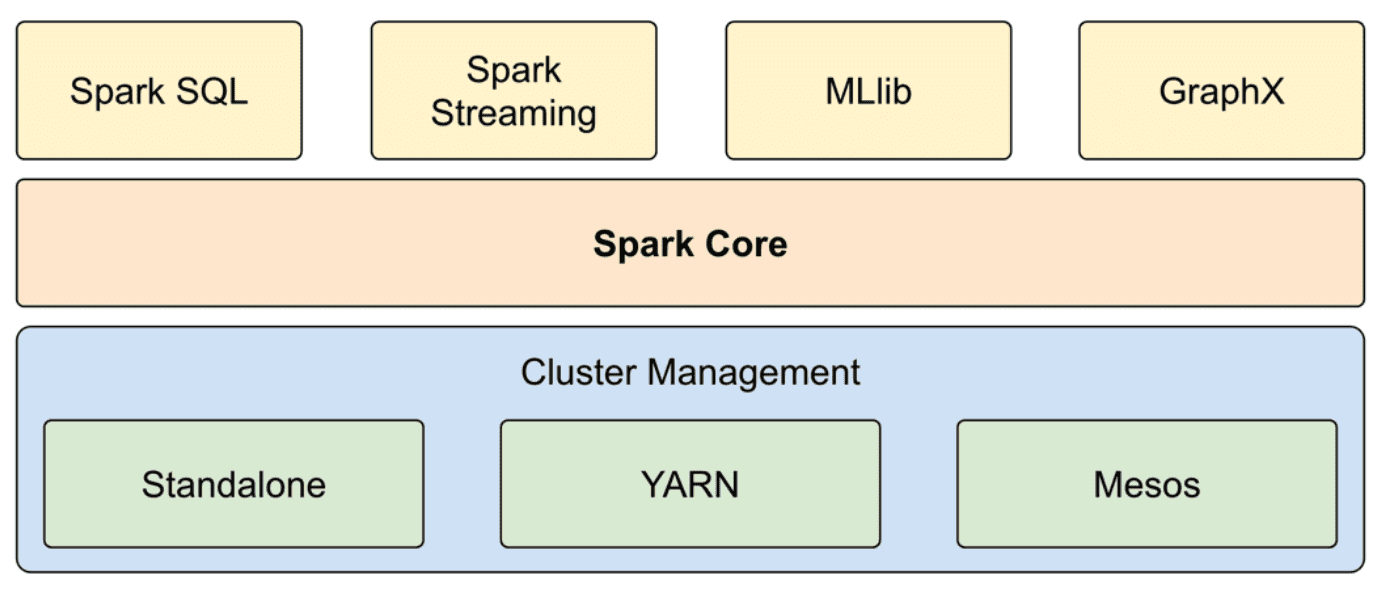
\includegraphics[width=1\linewidth]{img/sparkModules.png}
	\caption{Archiettura di Spark. Immagine tratta da \url{https://docs.incorta.com/}.}
	\label{fig:SparkModules}
\end{figure}
\par Vista la varietà di funzionalità che Spark offre, in questo progetto ci si focalizzerà maggiormente sulle funzionalità di SparkCore e sulle modalità di gestione di Streaming di dati. In entrambi i casi l'analisi verrà svolta sia da un punto di vista estereriore di quello che offre il framework che da quello interiore, andando a sviscerare le caretteristiche e i punti peculiari (positivi o negativi) che emergono dall'analisi. 
\newline
Si sottolinea che in questo progetto è stata utilizzata l'ultima versione disponibile di Spark, ovvero la \textbf{2.4.4}, in \textit{Scala}. Per cui per maggiori dettagli si rimanda alla relativa pagina di Spark \cite{spark}.
\subsection{Perchè Spark è così importante?}
L'importanza di Spark è data soprattutto dal fatto che in un unico framework vengono create intersezioni di vario genere che fanno sì che esso sia una piattaforma a tutto tondo. I seguenti punti sintetizzano i motivi principali dell'importanza di Spark.
\begin{itemize}
	\item Astrae la programmazione parallela: non sembra di lavorare su un cluster di computer.
	Nello scenario migliore sembrerà di lavorare con un database (SQL), nel peggiore di lavorare su Collections.
	\item Piattaforma unificata, tutto in un singolo framework.
	\item Facile da usare, leggere e capire.
\end{itemize}
\subsection{Un primo approccio a Spark}
Per prendere confidenza con Spark, così come abbiamo fatto con Scala, può essere utile utilizzare un'estensione della REPL di Scala per Spark (anche nota come \textbf{spark-shell}). 
Utilizzarla con Spark è molto semplice:
\begin{itemize}
	\item basta andare nell'url \url{https://spark.apache.org/downloads.html} e scaricare l'ultima versione di Spark (compresa di Hadoop);
	\item decomprimere la cartella e posizionarsi all'interno di essa da terminale;
	\item a questo punto, lanciando il comando \texttt{./bin/spark-shell} partirà la shell.
\end{itemize}
Si può anche memorizzare questo percorso nel path di sistema e accedervi da qualsiasi parte del file system. Aggiungendo a \texttt{$\sim$/.bashrc}:
\begin{itemize}
	\item \texttt{export SPARK\_HOME="percorso della cartella decompressa"} 
	\item \texttt{export PATH=$PATH:$SPARK\_HOME/bin:\$SPARK\_HOME/sbin}
\end{itemize}
Nella spark-shell vi sono già :
\begin{itemize}
	\item un'instanza di \texttt{SparkSession} \ref{sec:SparkSession} nominata \textit{spark};
	\item un'instanza di \texttt{SparkContext} \ref{sec:SparkContext} nominata \textit{sc};
	\item l'importazione dei moduli:
	\begin{itemize}
		\item \texttt{spark.implicits.\_}: per avere a disposizione una serie di impliciti utili nella lettura e nella manipolazione dei dati facenti parti della SparkSession;
		\item \texttt{spark.sql}: per operare con dati strutturati (SparkSQL).
	\end{itemize}
\end{itemize}
Seguendo il tutorial \cite{localexample} è possibile mettere le mani in pasta in locale su un dataset, esplorare le potenzialità di Spark (in particolare Spark SQL) e, soprattutto, del DLS che esso fornisce.
\subsubsection{SparkContext}\label{sec:SparkContext} 
Uno SparkContext è il punto di accesso ai servizi di Spark e, quindi, il fulcro di un'applicazione Spark. Infatti, un'applicazione Spark può essere considerata tale quando usa (direttamente o non) un'instanza di questa classe.
\newline
Esso imposta i servizi interni e stabilisce una connessione a un'ambiente di esecuzione Spark.

Uno SparkContext è essenzialmente un client dell'ambiente di esecuzione di Spark e funge da master dell'applicazione Spark (da non confondersi dal concetto di master in Spark, che verrà spiegato in seguito). Tra le funzionalità principali ci sono:
\begin{itemize}
	\item capire lo stato corrente dell'applicazione;
	\item impostare la configurazione;
	\item creare entità distribuite:  creare RDD \ref{sec:RDD}, broadcast e accumulators \ref{sec:broadcastAndAccumulators};
	\item accedere ai servizi di Spark;
	\item gestione dei jobs;
	\item gestione della persitenza.
\end{itemize}
Per ciascuna JVM ci può essere al più uno \textit{SparkContext}.
Per creare uno SparkContext potrebbe essere necessario fornire una configurazione che nel caso generale corrisponde a SparkConf, nel codice sottostante viene mostrato come creare uno SparkContext con una configurazione.

\lstinputlisting[language=Scala, firstline=9, lastline=12,basicstyle=\small]{../src/main/scala/it/unibo/pps18/spark/QuickStartBasic.scala}
La configuarazione imposta il nome dell'applicazione (\texttt{setAppName}) e il tipo di esecuzione con \texttt{setMaster} (di questo punto si discuterà in seguito). Queste due opzioni sono quelle necessarie da configurare, altre riguardano principalemente la personalizzazione dell'ambiente di esecuzione (vedi documentazione). In particolare, in questo caso viene configurato per usare hdfs.
Esistono altri costruttori per creare uno SparkContext. Quella con la SparkConf, a mio avviso, risultà più fluente delle altre modalità.
\subsubsection{SparkSession}\label{sec:SparkSession} 
SparkSession è il punto di accesso per lavorare con dati strutturati (API DataFrame e Dataset), in genere si opera attraverso un builder dal quale poi si ottiene l'istanza mediante \texttt{getOrCreate}. 
Nell'esempio sottostante viene mostrato il suo utilizzo, è molto simile all'esempio dello SparkContext.
\lstinputlisting[language=Scala, firstline=9, lastline=12,basicstyle=\small]{../src/main/scala/it/unibo/pps18/spark/QuickStartSparkSQL.scala}

Nota: esiste una vecchia versione dello SparkContext per il modulo dei dati strutturati chiamata \textit{SQLContext}, essa è stata lasciata per compatibilità ed è stata superata dalla SparkSession.
\section{Internals}
Essendo l'architettura interni di Spark molto grande, ci si concentrerà sulle parti principali e per maggiorni dettagli si rimanda a un \textit{gitbook} \cite{internals} che è risultato molto utile nella comprensione di questo tema.
\subsection{Architettura}
É possibile lanciare Spark essenzialmente in \textbf{due modalità}:
\begin{enumerate}
	\item \textbf{Interattiva (spark-shell)}: si tratta di un potente strumento per analizzare in modo interattivo e controllare lo stato delle attività nel Cluster. Non è raccomandabile usarlo in scenari reali.
	\item \textbf{Submit di un job}: da command line, non supporta altri casi come l'avvio di Spark da altre applicazioni anche se lo snippet di codice non è un jar (in caso di produzione).
\end{enumerate}
Queste modalità ci aprono al concetto di \textit{master-worker} (PCD) che nel ``dialetto di Spark" è noto come \textbf{``driver-executor"}.
\begin{figure}[H]
	\centering 
	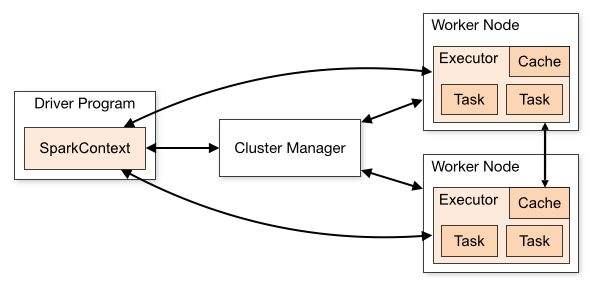
\includegraphics[width=1\linewidth]{img/cluster-overview.png}
	\caption{Driver-executor in relazione a Cluster Manager. Immagine tratta da \cite{spark}.}
	\label{fig:driverexecutor}
\end{figure}
Essenzialmente è possibile usare Spark con o senza un vero cluster (questo viene impostato nella \textit{SparkConf}):
\begin{itemize}
	\item \textbf{local mode}: uso in fase esplorativa per iniziare ad usare spark senza un effettivo cluster.
	\item \textbf{con cluster}:
	\begin{itemize}
		\item \textbf{client mode}: il driver è nel client, per cui è preferibile usarla in fase di debug;
		\item \textbf{cluster mode}: il driver è nel cluster, la uso in produzione.
	\end{itemize}
\end{itemize}
Quando si esegue Spark, lo stato dei processi è visibile in una pagina web che viene linkata nel esecuzione del progesso (la \textbf{Spark UI}), in essa è possibile visualizzare come viene effettivamente distribuito il lavoro, lo stato del lavoro e i DAG \ref{sec:DAG}. 

\par Nel caso in cui si utilizzasse un cluster c'è da porsi una domanda: \textit{``Chi controlla il cluster? Come Spark ottiene le risorse per driver e executor?"}
\newline La risposta è, come mostrato in Figura \ref{fig:driverexecutor}: il \textit{cluster manager}, come si nota in Figura \ref{fig:SparkModules}, fa parte dell'architettura di Spark ma non viene offerto da Apache Spark. Tra i più noti nel mercato abbiamo:
\begin{itemize}
	\item\textbf{Apache YARN\footnote{\url{http://hadoop.apache.org/docs/stable/hadoop-yarn/hadoop-yarn-site/YARN.html}}}: il gestore delle risorse in Hadoop 2.
	\item\textbf{Apache Mesos\footnote{\url{http://mesos.apache.org}}}: generale che può anche eseguire Hadoop MapReduce e le applicazioni di servizio.
	\item\textbf{Kubernetes\footnote{\url{https://kubernetes.io}}}: un sistema open source per automatizzare la distribuzione, il ridimensionamento e la gestione di applicazioni containerizzate. Non ancora adatto per fasi di produzione.
	\item\textbf{Standalone\footnote{\url{https://spark.apache.org/docs/2.4.4/spark-standalone.html}}}: semplice, facile e veloce. Incluso in Spark, semplifica la configurazione di un cluster. Non ancora adatto per fasi di produzione. 
\end{itemize}

\subsection{RDDs  e tasks}
\subsubsection{Resilient Distributed Datasets (RDDs)}\label{sec:RDD}
Spark ruota attorno al concetto di RDD, ovvero una collection fault-tollerant che può essere processata in parallelo. Ci sono due modi per creare un RDD: parellelizzando una collezione esistente nel driver program o facendo riferimento ad un archivio di dati esterno (come filesystem condivisi, HDFS, Hbase o qualsiasi input che ha dati in formato Hadoop).

Ci sono due operazioni fondamentali che vengono fatte sui dati, che rispecchiano essenzialemente il principio \textit{map-reduce}:
\begin{itemize}
	\item \textbf{transformations}: ovvero operazioni di \textit{map}, sono lazy: l'eventuale azione su di essa applicherà la trasformazione. Eventualmente è possibile rendere questi cambiamenti persistenti (con l'opportuno \texttt{persist}), altrimenti non lo sono.
	\item \textbf{actions}: ovvero operazioni di \textit{reduce}.
\end{itemize}
La Figura \ref{fig:RDDs} mostra l'intero meccanismo di RDDs e trasformazioni e azioni.
\begin{figure}
	\centering 
	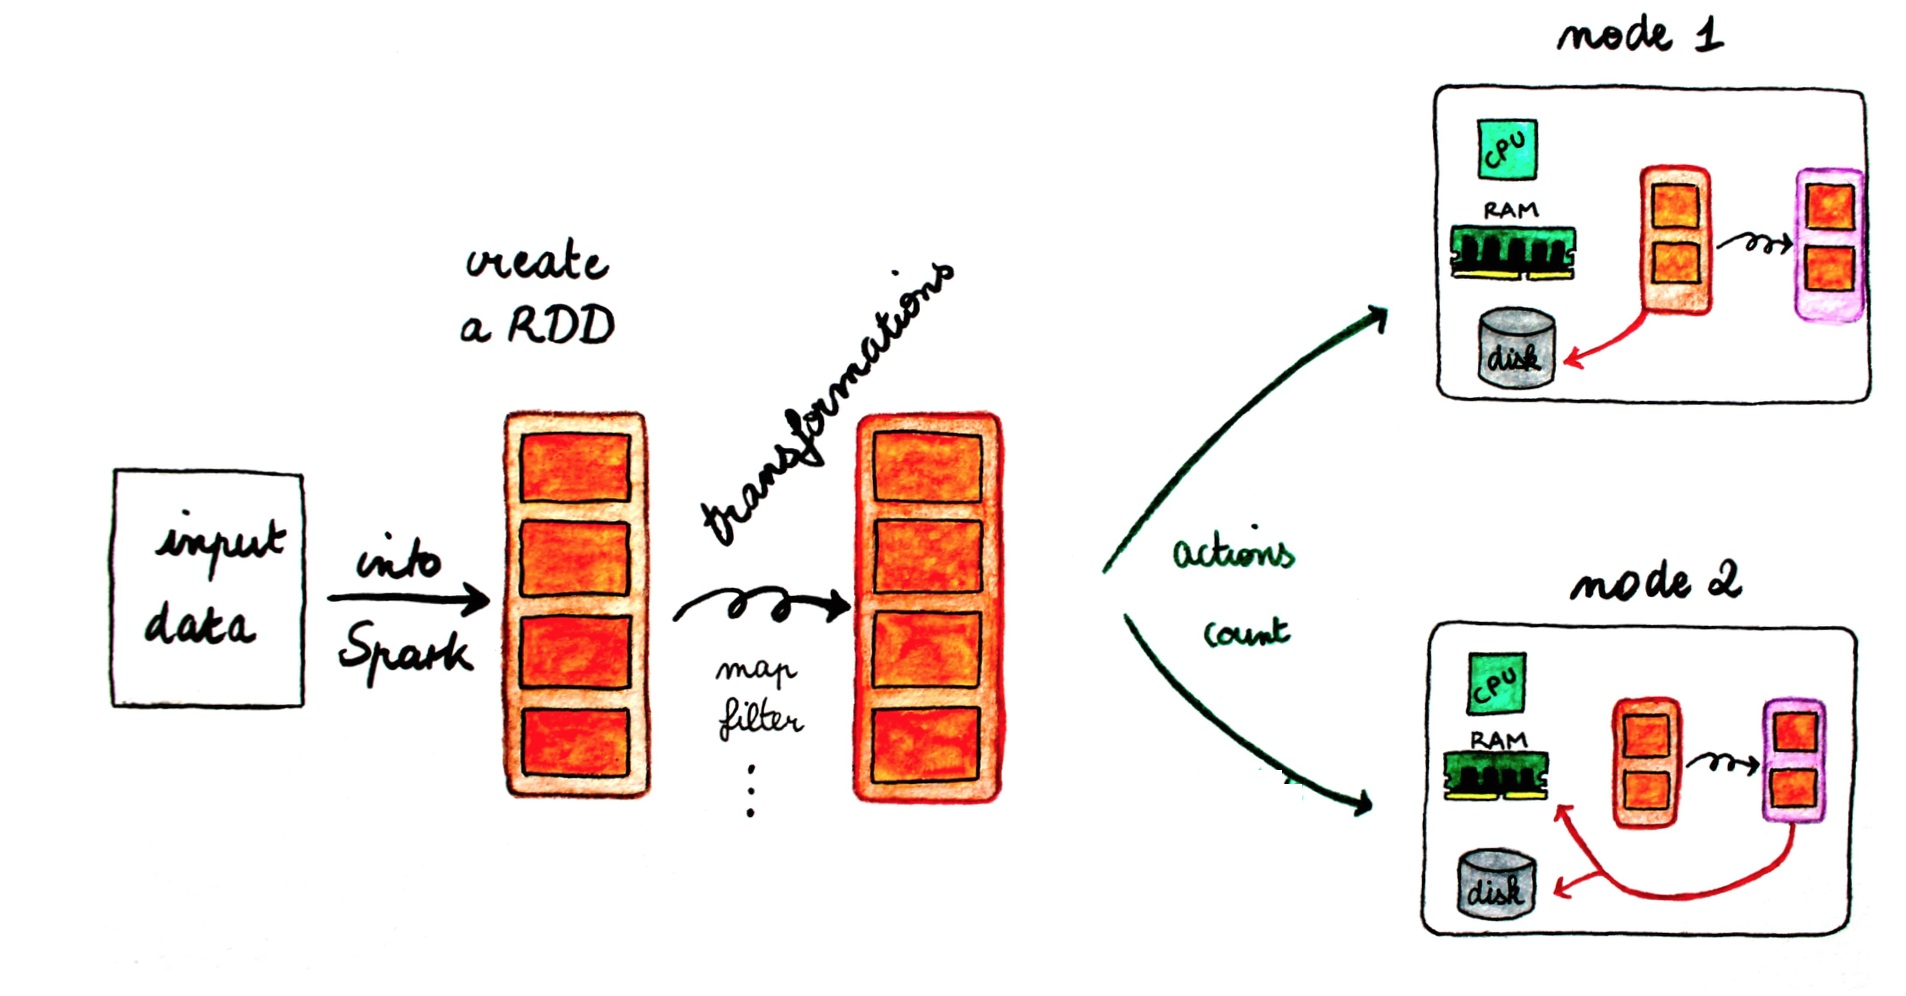
\includegraphics[width=1\linewidth]{img/rdds.png}
	\caption{RDDs e meccanismo di trasformations e actions. Immagine tratta da \url{http://sparkforbeginners.blogspot.com}.}
	\label{fig:RDDs}
\end{figure}
\subsubsection{Broadcast e Accumulators}\label{sec:broadcastAndAccumulators}
 Una delle cose più difficili di Spark è comprendere l'ambito e il ciclo di vita di variabili e metodi quando si esegue il codice in un cluster. Le operazioni RDD che modificano le variabili al di fuori del loro ambito di applicazione possono essere una fonte frequente di confusione. C'è sostanzialmente un problema di concorrenza e della \textit{closure} rispetto all'ambito di lavoro di un task che Spark risolve con l'inserimento di due concetti:
\begin{enumerate}
	\item \textbf{broadcasts}:  consentono al programmatore di mantenere una variabile di sola lettura memorizzata nella cache su ogni macchina anziché inviarne una copia con le attività. Possono essere utilizzati, ad esempio, per fornire ad ogni nodo una copia di un set di dati di input di grandi dimensioni in modo efficiente. Spark tenta anche di distribuire variabili di trasmissione utilizzando algoritmi di trasmissione efficienti per ridurre i costi di comunicazione.
	\item \textbf{accumulators}: sono variabili che vengono “aggiunte” solo attraverso un'operazione associativa e commutativa e possono, quindi, essere supportate efficientemente in parallelo. Possono essere utilizzati per implementare contatori (come in MapReduce) o somme. Spark supporta nativamente accumulatori di tipi numerici e i programmatori possono aggiungere il supporto per nuovi tipi. Vale sempre il concetto lazy (vedi trasformazioni).
\end{enumerate}

\subsubsection{RDDs e conseguenze}
Poichè Dataset e DataFrame (API di dati strutturati) ereditano da RDDs (non strutturati), capendo questi ultimi possiamo capire come effettivamente viene distribuito il lavoro tra gli executors.

Quando viene letto un file è possibile specificare il numero di \textbf{partizioni di un RDD} che (guarda caso) coincide con il corrispondente \textbf{numero di task}.
Ovviamente, numero executors e di task sono effettivamente correlati e quindi bisogna specificare il numero di conseguenza.

Si lavora in \textbf{stage}, uno stage rappresenta un periodo (una o più funzioni chiamate sui dati) in cui non è necessario uno shuffle, ovvero non è necessario spostare i dati tra le partizioni (\textbf{data locality}). Se i dati devono muoversi (es. reduceByKey) bisogna ripartizionarli (\textit{shuffle \& sort}).
Con \textit{collect} si ritorna dagli executor al driver.

\subsubsection{DAG (Directed Acyclic Graph) }\label{sec:DAG}
Un \textbf{DAG} è un grafo diretto senza cicli, dove i nodi rappresentano gli RDD e gli archi le operazioni da applicare su questi ultimi. Un esempio di DAG è mostrato in Figura \ref{fig:DAG}.
A fronte della chiamata di un'azione, il DAG creato viene inviato al DAG Scheduler che suddivide ulteriormente il grafo negli stage delle attività.
\par Un DAG consente all'utente di comprendere effettivamente cosa sta accadendo, anche in merito agli shuffle e gli stage.
\begin{figure}[H]
	\centering 
	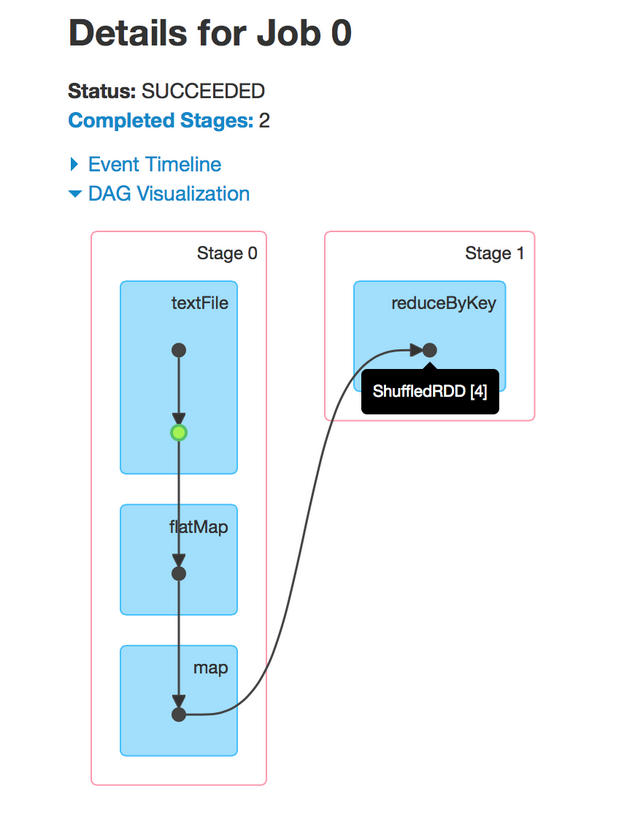
\includegraphics[width=0.8\linewidth]{img/DAG.png}
	\caption{Esempio DAG di Spark. Immagine tratta da \url{https://databricks.com}.}
	\label{fig:DAG}
\end{figure}
\subsection{Modello di esecuzione} 
Il modello di esecuzione di Spark, visibile - durante l'esecuzione - nel dettaglio nella Spark UI (http://:4040), può essere diviso nelle seguenti macro-fasi (come mostrato in Figura \ref{fig:model}):
\begin{enumerate}
	\item \textbf{creazione del piano logico};
	\item \textbf{traduzione del piano logico in un piano fisico};
	\item \textbf{esecuzione delle attività sul cluster}.
\end{enumerate}
Nel caso in cui si volesse visualizzare, ad esecuzione terminata, il dettaglio grafico è possibile visitare la \textit{Spark history} (http://:18080).
\begin{figure}[H]
	\centering 
	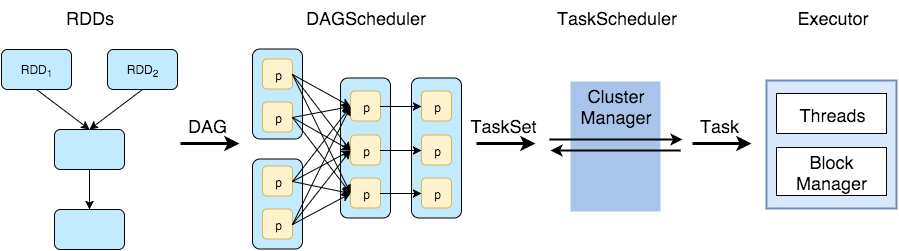
\includegraphics[width=1\linewidth]{img/model.png}
	\caption{Job scheduling in Spark. Immagine tratta da \url{http://datastrophic.io}.}
	\label{fig:model}
\end{figure}
Nel dettaglio le fasi sono le seguenti:
\begin{itemize}
	\item crea DAG e RDDs per rappresentare la computazione;
	\item crea il piano di esecuzione logico del DAG;
	\item fa pipeline il più possibile;
	\item divide in \textbf{stages};
	\item schedula e esegue i tasks;
	\item divide ogni stage in task;
	\item task = dati + computazione;
	\item esegue tutti i task di uno stage prima di andare avanti.
\end{itemize}

\subsection{Di più sullo shuffle}
Note importanti e aggiuntive sullo shuffle sono:
\begin{enumerate}
	\item è pull based e non push based;
	\item scrive file intermedi nei dischi.
\end{enumerate}
Bisogna tenere d'occhio il \textbf{numero di partizioni} perchè possono fondamentalmente crearsi due situazioni:
\begin{enumerate}
	\item numero troppo \textbf{basso}:
	\begin{itemize}
		\item poca concorrenza;
		\item più suscettibile a \textit{``data skew"} (spostamento di dati);
		\item maggiore uso della memoria in operazioni che richiedono Shuffle (groupBy, sortByKey, reduceByKey, etc.).
	\end{itemize}
	\item numero troppo \textbf{alto}: problemi opposti, dati troppo sparsi e non viene sfruttato il partizionamento.
\end{enumerate}
Un numero appropiato di solito è tra 100 e 10000.
Bisogna fissare questo numero nell'intervallo compreso tra:
\begin{itemize}
	\item \textbf{lower bound}:  almeno circa il doppio del numero di core di un cluster;
	\item \textbf{upper bound}: essere sicuri che un task venga eseguito in almeno 100ms.
\end{itemize}
Quindi analizzando Spark UI e dai DAG, si capisce cosa effettivamente sta succedendo nel Cluster e si comprende quale soluzione sia la migliore. Non è detto che la soluzione migliore in termine di movimenti di dati sia quella con un codice più compatto ed ``esteticamente" migliore.
\section{Moduli di Spark}
Bisogna sottolineare che le applicazioni \textit{Scala} dovrebbero definire un metodo \texttt{main()} anzichè estendere \texttt{scala.App}. Le sottoclassi di \texttt{scala.App} potrebbero non funzionare correttamente \cite{spark}.
\subsection{Iniziare a lavorarare con Spark e gli RDDs}
Gli RDD, introdotti nella sezione precendente, rappresentano la base di ciò che offre Spark con il modulo SparkCore. In questa sezione si parlerà degli aspetti esteriori di questo concetto e di come utilizzarli.
\par Per passare funzioni a Spark nella documentazione viene mostrato come sfruttare map su un RDDs applicando una propria funzione che prende in input un dato dello stesso tipo di quello contenuto nel RDDs. Questo aspetto da un lato obbliga il programmatore ad appoggiarsi alle API fornite dal framework e quindi ottimizzate da Spark, dall'altro pone dei limiti nel come il programmatore vuole approcciarsi ai dati; limiti che vengono ridotti dalla potenza e dalla facilità di comprensione del DLS che Spark mette a disposizione, soprattutto nel modulo SparkSQL.
\par Per quanto riguarda il \textbf{caching}, oltre a \texttt{persist}, esistono modalità per specificare a quale memoria far riferimento e funziona anche su dati presenti in molti nodi.
\par Se si andasse ad applicare \texttt{collect()} su una grande quantità di dati potrei incorrere in un \textit{``out of memory"}, per cui bisogna applicare concetti simili a quelli visti durante il corso di PPS. Ad esempio anzichè fare una stampa di tutti i dati, si vanno recuperare i primi N record con una \texttt{take(N)}.
\par Un esempio di utilizzo di SparkCore senza l'ausilio di ulteriori moduli è presente nella classe \texttt{/src/main/scala/it/unibo/pps18/spark/QuickStartSparkBasic.scala}, nel quale viene interrogato un container docker (\texttt{src/main/docker/basic-container})  con dati in HDFS in formato \textit{csv}. Nell'esempio vengono messi in evidenza i limiti che si incontrano nel caso in cui non si utilizzino altri moduli di supporto (questo punto verrà compreso meglio nella sezione su SparkSQL \ref{sec:SparkSQL}).
\subsection{Machine Learning Library (MLlib)}
Questo modulo consiste in:
\begin{itemize}
	\item \textit{Algoritmi di Machine Learning}: come classificazione, regressione, clustering e filtering collaborativo.
	\item \textit{Featurization}: estrazione delle feature, transformazione, riduzione della dimensionalità e selezione.
	\item \textit{Pipelines}: tool per costruire, valutare e fare tuning di pipeline di ML.
	\item \textit{Persistenza}: salvare e eseguire algoritmi, modelli e pipeline.
	\item \textit{Utility}: algebra lineare, statistica, gestione dati, etc.
\end{itemize}
\subsection{GraphX Programming}
Componente Spark per Grafi e calcolo graph-parallel.

Ad alto livello viene estratto il concetto di RDD introducendo l'estensione Graph, in Figura \ref{fig:GraphX} viene mostrata la costruzione del grafo a partire dai dati grezzi.
Ci sono varie operazioni a supporto di questo concetto, anche algoritmi e builder per l'analisi.
\begin{figure}[H]
	\centering 
	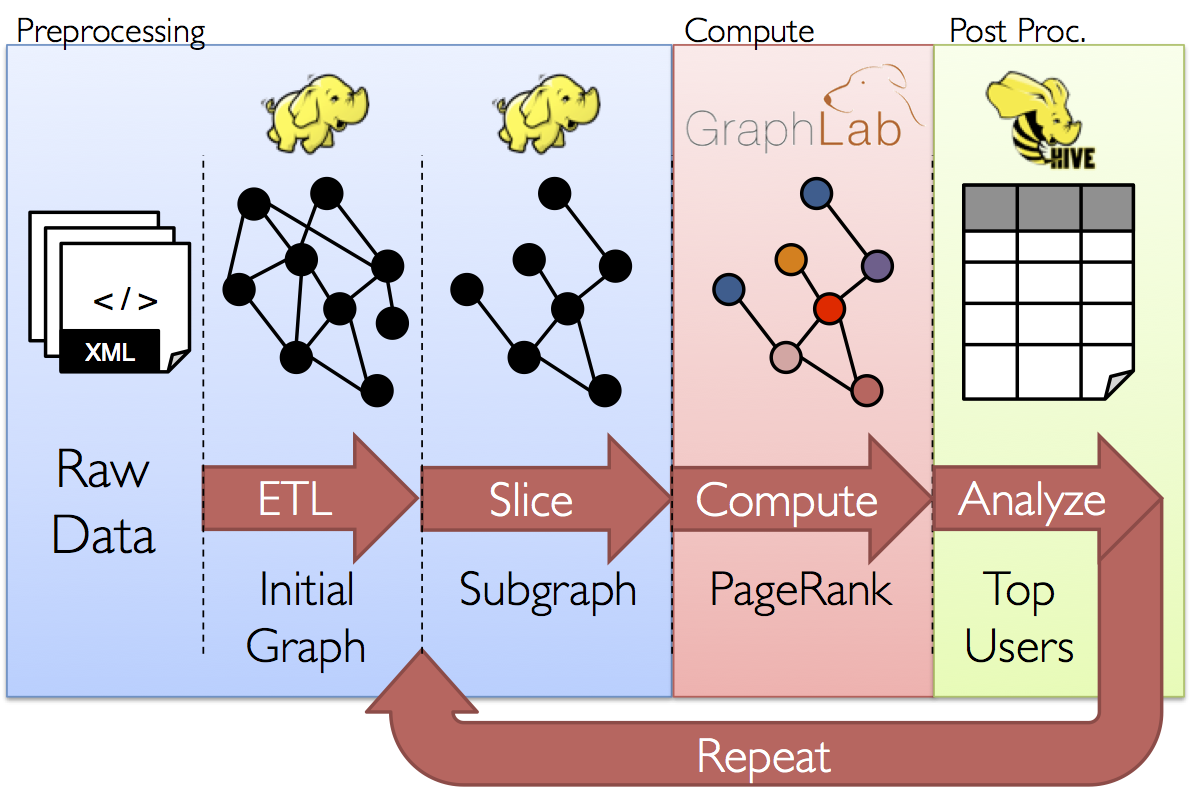
\includegraphics[width=0.8\linewidth]{img/graph_analytics_pipeline.png}
	\caption{Funzionamento di GraphX. Immagine tratta da \cite{spark}.}
	\label{fig:GraphX}
\end{figure}
Nello specifico si consiglia di utilizzare questa estensione quando nella natura dei dati ci sono legami che vengono meglio rappresentati da un grafo.
Prima di dare in pasto i dati a GraphX potrebbero servire minime operazioni per renderli ``compatibili" con la visione a grafo.
Nella costruzione vengono richiesti:
\begin{itemize}
	\item RDD dei vertici;
	\item RDD degli edge;
	\item un vertice di default (pozzo).
\end{itemize}
\subsection{SparkR (R on Spark)}
SparkR è un pacchetto R che fornisce un frontend leggero per utilizzare Apache Spark da R. In Spark 2.4.4, SparkR fornisce un'implementazione di Dataframe distribuiti che supporta operazioni come selezione, filtro, aggregazione ecc. (simile a data frame R, dplyr \footnote{\url{https://www.rdocumentation.org/packages/dplyr}}), ma su set di dati di grandi dimensioni. SparkR supporta inoltre l'apprendimento automatico distribuito tramite MLlib.

\subsection{Spark SQL}\label{sec:SparkSQL}
Modulo di supporto a dati strutturati, fornisce maggiori ottimizzazioni rispetto a RDD. L'interazione con i dati è possibile in vari modi, tra cui SQL e Dataset API.
Nella computazione viene usato un unico engine di esecuzione, il programmatore può esprire le interrogazioni nel modo che ritiene più naturale. É possibile fare uso di Hive, JDBC, etc. 
\newline
Di seguito verranno analizzati gli aspetti più interessanti e pratici, di questo modulo.
\par Alcuni benchmarks\footnote{\url{https://blog.knoldus.com/spark-rdd-vs-dataframes}} dimostrano che i DataFrame sono più ottimizzati in termini di elaborazione, forniscono più opzioni per aggregazioni e altre operazioni con una varietà di funzioni disponibili (molte più funzioni sono ora supportate nativamente in Spark 2.4) rispetto agli RDD.
\subsubsection{Dataset API}
Operazioni con cui interrogare il Dataset. 
\par Nota interessante, in Scala, DataFrame è così definito ``type DataFrame = Dataset[Row]" \cite{spark}.
\par Un Dataset si può creare anche ``on the fly" da un file di testo o appartenere a determinati formati (es. Hadoop HDFS) o trasformando altri Dataset.
Nelle interrogazioni che lo richiedono vengono passate funzioni, questi aspetti verranno meglio sviscerati nella sezione sullo Streaming Strutturato \ref{sec:structuredstreaming}.
\par In \texttt{/src/main/scala/it/unibo/pps18/spark/QuickStartSparkSQL.scala} viene mostrato come l'utilizzo di queste API renda maggiormente fluente le interrogazioni su un container docker (\texttt{src/main/docker/basic-container}) con dati in HDFS in formato \textit{csv}.
\newline 
Le stesse interrogazioni, senza il supporto dell'API SparkSQL, ma del solo SparkCore, sono sicuramente meno leggibili e, come mostrato nel corrispondente esempio di utilizzo presente in \texttt{/src/main/scala/it/unibo/pps18/spark/QuickStartBasic.scala}, portano a dover gestire problematiche di basso livello, sia a livello di interrogazioni che di parsing dei file. Queste problematiche (a questo livello) non dovrebbero interessare il programmatore, vengono efficientemente superate e gestite dal modulo SparkSQL.

\subsection{Moduli per lavorare con stream di dati}
Attualmente è molto importante considerare dati provenienti da stream real time, di varia natura. Questo aspetto sta diventando sempre più una sfida complessa che si associa in modo naturale ai \textit{Big Data} e alla sempre più fondamentale necessità di trarre informazioni dai dati e utilizzarli per prendere decisioni importanti dal punto di vista aziendale. \newline
Spark si avvicina a questo mondo con due moduli: \textbf{Spark Streaming} e \textbf{Spark Structured Streaming}. I quali verranno descritti e analizzati nelle seguenti sezioni.
\subsubsection{Spark Streaming}
Spark Streaming, come mostrato in Figura \ref{fig:SparkStreaming}, raccoglie dati provenienti da varie fonti (es. Kafka, Flume, Kinesis o TCP sockets, file) e li processa usando algoritmi complessi espressi attraverso funzioni high-level come \textit{map}, \textit{reduce}, \textit{join} e \textit{window}. Infine, il risultato prodotto può essere inserito in File Systems (HDFS), Databases o Dashboard da eventualemente elaborare con le funzioni di Spark ML e Graph.
\begin{figure}[H]
	\centering 
	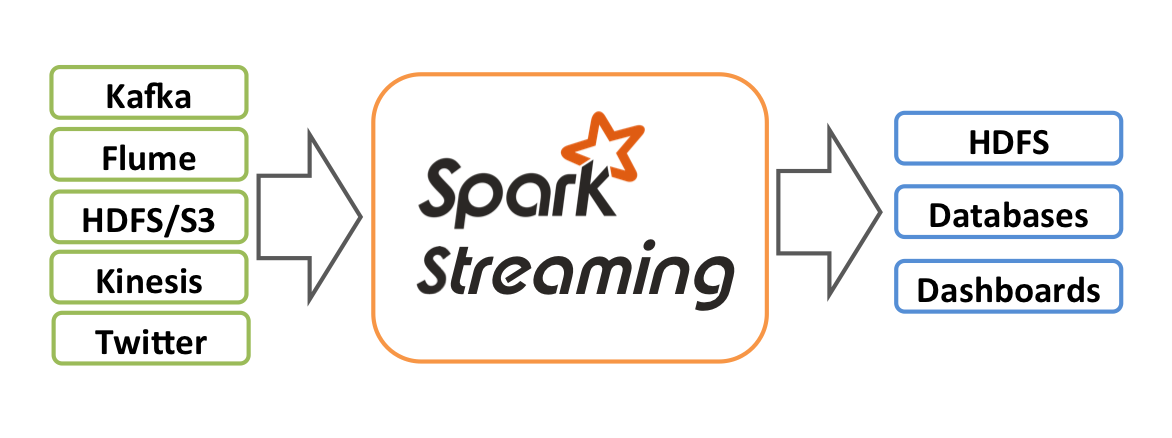
\includegraphics[width=1\linewidth]{img/sparkStreaming.png}
	\caption{Funzionalità di Spark Streaming. Immagine tratta da \cite{spark}.}
	\label{fig:SparkStreaming}
\end{figure}
\par Internamente Spark Streaming, come mostrato in  Figura \ref{fig:SparkStreamingBatch}, divide lo stream in batch di dati che vengono processati dalla Spark Engine.
\newline
La lettura di uno stream avviene tramite un \textbf{Receiver} ed eredita dall'astrazione \textbf{DStream}, si tratta di dati che provengono da varie fonti (es. Kafka, Flume, and Kinesis) o da operazioni ad alto livello su altri DStream.
Un DStream può essere considerato come una sequenza di RDDs.
\begin{figure}[H]
	\centering 
	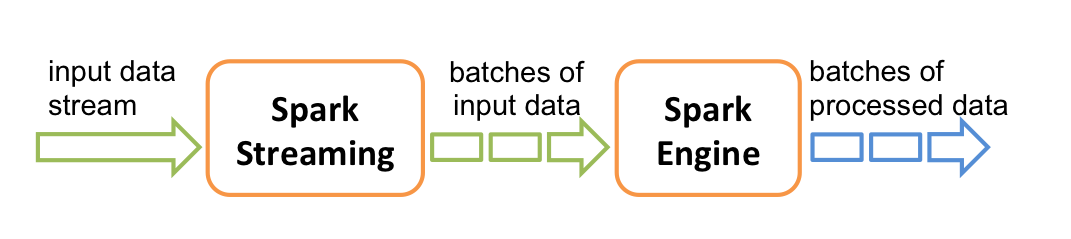
\includegraphics[width=1\linewidth]{img/sparkStreamingBatch.png}
	\caption{Divisione micro-batch in Spark Streaming. Immagine tratta da \cite{spark}.}
	\label{fig:SparkStreamingBatch}
\end{figure}
Fondamentale è la definizione di un \textbf{batch interval}, esso indica la durata secondo la quale uno Spark Streaming Job immagazzina dati e, per cui, in ogni intervallo ci sarà un DStream differente.
Questo concetto fa capire la forte nota di Spark Streaming nel lavorare in micro batch e non in real time, questo è essezialmente per maggiori performance \footnote{\url{https://sqlstream.com/5-reasons-why-spark-streamings-batch-processing-of-data-streams-is-not-stream-processing/}}.

Le \textbf{operazioni su un DStream}, molto simili a quelle su un RDD, funzioni proprie si possono applicare 
solo attraverso quelle fornite dall'API, questo è limitante rispetto allo Structured Streaming \ref{sec:structuredstreaming}.

\par Per usare Spark Streaming è necessario definire uno \textbf{SparkStreamingContext} (specializzazione dello StramingContext per questo modulo), per il quale bisogna definire uno \textit{StreamingContext} e un \textit{BatchInterval}.
Attraverso dei metodi preposti in questa struttura verranno consumati dati e creati di conseguenza i relativi DStream.

\par A volte non basta considerare un intervallo, ma è più opportuno considerare una finestra, per cui si passa da una transformazione \textit{stateless} (in cui vengono scartati dati provenienti da batch precedenti) a una trasformazione \textit{stateful}. In particolare, con lo \textbf{sliding windows} vengono aggregati DStream appartanenti a intervalli diversi.
Ci sono due ulteriori parametri, oltre al batch interval, da tarare:
\begin{itemize}
	\item \textbf{window size}: multiplo di batch interval, indica l'ampiezza temporale della finestra;
	\item \textbf{slide window dimension}: indica quanta distanza temporale c'è tra una window e la successiva, anche esso è multiplo del batch interval e potenzialmente potrebbero esserci finestre sovrapposte.
\end{itemize}
Un'esempio grafico di quello che accade con questo genere di trasformazioni è mostrato in Figura \ref{fig:StructuredStreaming}.
\begin{figure}[H]
	\centering 
	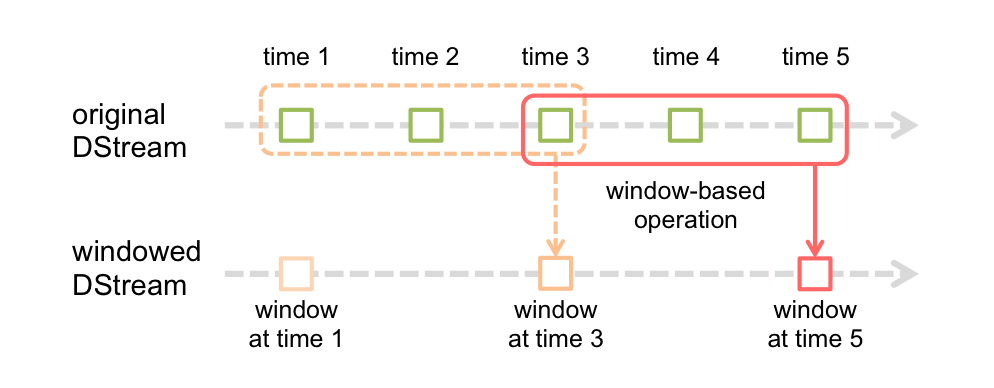
\includegraphics[width=1\linewidth]{img/sparkStreamingWindow.png}
	\caption{Divisione dei DStream in finestre temporali. Immagine tratta da \cite{spark}.}
	\label{fig:SparkStreamingWindow}
\end{figure}
\par Una nota di rilevanza fondamentale nello streaming e non supportata da questo modulo è che esso non riesce a lavorare con il tempo dell'evento, ma solo con quello dell'evento di Spark.
\par Per la gestione degli errori con questo modulo è necessario replicare i dati in altri supporti (es. Kafka).
\par Con Spark Streaming non ci sono restrizioni per utilizzare qualsiasi tipo di sink, ovvero fonti esterne su cui esportare il risultato di operazioni di aggregazioni sui dati provenienti dagli Stream. Infatti, attraverso il metodo ``\texttt{foreachRDD}" è possibile accedere ai dati del DStream e farci essenzialmente qualsiasi cosa. 

\par Un esempio di utilizzo del modulo è presente in \texttt{/src/main/scala/it/unibo/pps18/spark/streaming/SparkStreaming.scala}, nel quale vengono creati dei Receiver di stream di dati infiniti e vengono effettuate operazioni di vario genere per capire fino a che punto ci si può spingere con questo modulo e cosa offre. I limiti riscontrati, in confronto con il nuovo modulo Structured Streming \ref{sec:structuredstreaming}, sono notevoli e verranno discussi nella seguente sezione.

\par Inoltre, si è cercato di comprendere le differenze di questo modulo rispetto ad altri framework e librerie per la gestione dello streaming \footnote{\url{https://medium.com/@chandanbaranwal/spark-streaming-vs-flink-vs-storm-vs-kafka-streams-vs-samza-choose-your-stream-processing-91ea3f04675b}}. Nello specifico:
\begin{itemize}
	\item \textbf{Apache Storm}\footnote{\url{https://www.slideshare.net/ptgoetz/apache-storm-vs-spark-streaming}} \footnote{\url{https://www.educba.com/apache-storm-vs-apache-spark/}}: si tratta di un framework che processa nativamente stream di dati, con un modulo che offre anche la possibilità di lavorare in micro-batch (\textit{Trident}). Spark è totalmente differente: è un framework per processare batch di dati e aggiuntivamente, con il modulo SparkStreaming, lavora su stream di dati in micro-batch. Per cui il confronto tra i due mondi è poco applicabile, infatti a tutto ciò si inserisce il fatto che non esistono benchmark e configurazioni pubbliche di Spark e il paper relativo a SparkStreaming\cite{sparkStreaming} risulta antecedente di due anni rispetto allo sviluppo di Trident. Ci sono nette differenze tra Trident e SparkStreaming soprattutto nella gestione più occurata delle failure da parte di Trident, in termini di performance si dimostra che SparkStreaming sia 40x volte più veloce.
	Storm, inoltre, risulta più difficile da apprendere, da utilizzare e comprendere rispetto a Spark e l'ecosistema che offre Spark spesso viene preso in considerazione per avere una visone completa del contesto dei dati e non solo dello streaming.
	\item \textbf{Flink}: nativamente per lo streaming (similmente a Storm), ma con supporto anche a dati batch, molto simile a Spark. Infatti, sembra ci sia proprio una lotta per il primato con Spark nella quale Flink sembra superarlo, ma quest' ultimo sta recuperando punti con il modulo di Structured Streaming.
	\item \textbf{KafkaStream}: libreria \textit{light-weight} che può essere utilizzata in un'architettura a micro servizi. Facile da capire e da usare, con il vincolo di avere \textit{Kafka}. 
	\item \textbf{Samza}: simile a \textit{KafkaStream}, sviluppata dagli stessi sviluppatori. Samza è una specie di versione ridimensionata di Kafka Streams. Mentre Kafka Streams è una libreria destinata ai microservizi, Samza è un'elaborazione cluster completa che gira su Yarn.
\end{itemize}
Tirando le somme, la scelta della soluzione di streaming da utilizzare dipende dai casi. Nel caso di IoT, sistemi nativamente stream, come Kafka e Storm, sono altamente consigliati. Considerando cambiamenti a lungo termine potrebbe essere opportuno appoggiarsi su framework più completi, come Flink e Spark. Così come avere già altri parti di sistemi su Spark (o Flink) porta naturalmente ad usare i moduli offerti dal framework che già si sta utilizzando.
Inoltre, bisogna anche capire la garanzia dal punto di vista di aggiornamenti che vengono offerti; per questo punto Spark sembra sia molto attivo.
Con gli anni, come qualsiasi ambito informatico, le cose potrebbero cambiare: si stanno sviluppando tante altre soluzioni proprietarie e non, come rispettivamente \textit{Google Dataflow} \footnote{\url{https://cloud.google.com/dataflow/}} e \textit{Apache Apex} \footnote{\url{https://apex.apache.org}}.

\par In ogni caso nel mondo Spark, la tendenza, la novità e il maggior supporto sembra siano nel modulo ``\textit{Spark Structured Streaming}", il quale verrà discusso di seguito.
Nonostante ciò sembra continui ad esserci interesse per questo modulo, magari per dati senza una struttura ben delienata. Un esempio dei giorni d'oggi è l'uso di questo framework applicato al 5G \footnote{\url{https://www.ericsson.com/en/blog/2019/6/applying-the-spark-streaming-framework-to-5g}}.

\subsubsection{Spark Structured Streaming}\label{sec:structuredstreaming}
Streaming strutturato, costruito sopra a Spark SQL e dunque con supporto a DataFrame e Dataset. 
Sostanzialmente è possibile riuso totale del codice scritto per interrogazioni statiche su SparkSQL.
\par Non c'è il concetto di batch di Spark Streaming, assomiglia più a uno stream \textit{real time}.
In ogni caso sotto si procede per micro batch, dalla versione 2.3 di spark è stato aggiunto il concetto di \textit{Continuous Processing} che ha ridotto ulteriormente la latenza.
Nota interessante è che nell'approcciarsi al CP, Spark ha usato una versione adattata del noto algoritmo di Chandy-Lamport (visto in PCD) \footnote{\url{https://databricks.com/blog/2018/03/20/low-latency-continuous-processing-mode-in-structured-streaming-in-apache-spark-2-3-0.html}}.
\par I dati, come mostrato in Figura \ref{fig:StructuredStreaming}, vengono aggiunti a una tabella potenzialemente infinita, composta da una sola colonna ``value" (DataSet \textless Row\textgreater ),  la quale tramite le funzionalità di SparkSQL e opportuni interventi del programmatore nel definire classi che rispecchiano la struttura dei dati, verrà trasformata nelle colonne opportune.
É \textbf{importante} sottolineare che non viene materializzata l'intera tabella, man mano che vengono interrogati i dati vengono scartati. 
\begin{figure}[H]
	\centering 
	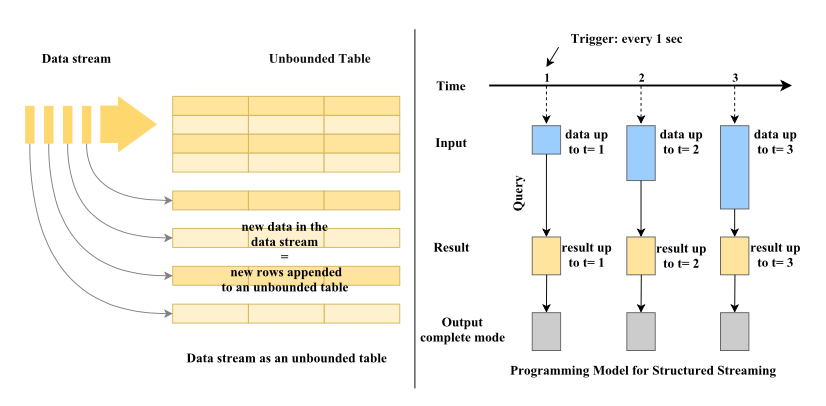
\includegraphics[width=1\linewidth]{img/sparkStructuredStreaming.png}
	\caption{Come Spark Structured Streaming mantiene i dati. Immagine tratta da \cite{structuredStreaming}.}
	\label{fig:StructuredStreaming}
\end{figure}
Per connettersi alle risorse dati bisogna:
\begin{itemize}
	\item Creare una \texttt{SparkSession};
	\item chiamare il metodo \texttt{readStream} su questa, che è effettivamente il metodo \texttt{read} di SparkSQL su uno streaming;
	\item \texttt{.format()} per specificare il tipo di dato (es. Kafka, Socket, File);
	\item \texttt{.options} per eventuali opzioni come host e porta.
\end{itemize}

I dati ottenuti possono avere come sink (chiamata al metodo \texttt{writeStream}): kafka, file, memoria, console.
Con Spark 2.4 lo Structured Streaming ha superato i limiti restringenti che aveva in precedenza sul numero di sink, introducendo un sink ``\texttt{foreachBatch}", questo fornisce la tabella di output risultante con DataFrame per eseguire operazioni custom.
\par I dati vengono ottenuti in ogni momento e la modalità con cui si recuperano può essere (dipendentemente dall'interrogazione): 
\begin{itemize}
	\item \textit{Complete}: per ottenere l'output completo di ogni aggiornamento;
	\item \textit{Append}: solo righe aggiunte;
	\item \textit{Update}: solo righe aggiornate.
\end{itemize}

Questo modello è molto differente da altre engine di streaming, molte richiedono all'utente stesso di mantenere aggregazioni sui dati precedenti e sulla loro coerenza.
In questo modello se ne occupa Spark e il tutto rimane trasparente all'utente.
Le modalità di triggering possono essere:
\begin{itemize}
	\item \textit{default o micro batch mode}: esegue il micro batch non appena possibile;
	\item \textit{fixed}: intervalli di micro batch fissati;
	\item \textit{one time}: eseguito una sola volta;
	\item \textit{continuous} con un intervallo di checkpoint fissato (sparimentale): continuos processing mode.
\end{itemize}

Le operazioni supportate nell'interrogazione ai dati che provengono dalla \texttt{readStream}, sono le seguenti:
\begin{itemize}
	\item funzioni di base di SparkSQL;
	\item \textbf{window based sliding}, molto simile a quello supportato da SparkStreaming,
	\item \textbf{UDF} \cite{internalsSQL} (\textit{user defined functions}): si tratta di normalissime funzioni Scala definite dall'utente, che si possono considerare come ``black box". Il tutto ha un senso unificato all'utilizzo di case class definite dall'utente rappresentative dei record appartenenti agli stream di dati.
	Le UDF sono registrabili anche globalmente nella sessione.
	Attenzione però ad all'utilizzo di UDF, bisogna vedere i piani di esecuzione, valutari e comprendere se effettivamente, essendo scatole nere, ottimizzano l'esecuzione o se essa può essere resa meno leggibile ma più performante, e comunque eseguibile, con i meccanismi offerti da Spark e dai suoi moduli. Inoltre, UDF ha problemi di seriazzazione, ogni volta deve deserializzare e serializzare le colonne, per cui quando possibile è consigliato preferire le funzioni builtin che in SparkSQL non sono poche \cite{spark}. 
	\item \textbf{UDAF} \cite{internalsSQL} (user-defined aggregate function) : si tratta di funzioni personalizzate che forniscono aggregazione, estensione di \texttt{UserDefinedAggregateFunctions}. Una UDAF riduce dimensionalmente i dati, a differenza di una UDF che effettua una trasfomazione uno a uno, e valgono le considerazioni fatte per le UDF. Non sono ancora supportate per lo streaming, ma funzionano per dati statici con SparkSQL.
\end{itemize}
Nell'abito delle \textbf{operazioni con stato arbitrarie}, esistono delle funzioni che permettono di usare le UDF su Dataset aggregati, per aggiornare lo stato definito dall'utente (\texttt{mapGroupsWithState} e \texttt{flatMapGroupsWithState}).

\par Per l'essenza dello streaming, in questo modulo non sono supportate alcune funzioni di SparkSQL \footnote{\url{https://spark.apache.org/docs/2.4.4/structured-streaming-programming-guide.html\#unsupported-operations}}.

\par Questo modulo, a differenza di Spark Streaming, riesce a lavorare con il \textbf{tempo dell'evento}. Per questo motivo è più adatto al mondo reale (es. IoT).
In caso di ritardi è Spark stesso a preoccuparsi di aggiornare e rimanere con l'event time corretto.
Da Spark 2.1 c'è il concetto di \textbf{watermarking} che permette all'utente di definire una soglia dei dati in ritardo, e consente, di conseguenza, all'engine di ripulire il vecchio stato.
Occhio alle dimensioni di questo valore, se troppo grande può creare problemi di memoria / performance. Questo è molto importante, delle tipologie di sink non lo supportano in update ma solo in append in modo  che tutto venga scritto alla fine.
\newline
Con tutti questi aspetti nasce il forte senso di Structured Streaming e il distacco rispetto a  Spark Streaming.
\par Spark Structured Streaming assicura ``\textit{end-to-end exactly-once semantics}" sotto ogni failure.
Oltre al checkpointing per ripristinare la condizione dagli errori, usato anche da Spark Streaming, usa due condizioni:
\begin{itemize}
	\item la fonte deve essere riproducibile;
	\item i sink devono supportare operazioni idempotenti per supportare il ritrattamento in caso di guasti.
\end{itemize}
\par Con questo modulo si possono fare \textbf{join} \footnote{\url{https://docs.databricks.com/_static/notebooks/stream-stream-joins-scala.html}} (inner, outer, etc.) incrementali con altri DataFrame o Dataset (su una colonna specifica), siano essi statici o non.
Ancora non c'è un supporto completo \footnote{\url{https://spark.apache.org/docs/2.4.4/structured-streaming-programming-guide.html\#support-matrix-for-joins-in-streaming-queries}}, infatti questa è una delle sfide di questo modulo: risulta difficile fare join su dati che sono incerti e che possono arrivare in qualsiasi momento. Come nello streaming, c'è un \textit{watermark delay} per mantenere i dati oppure una \textit{event-time range condition} per specificare che un certo dato può arrivare in un certo range di tempo.

\par Altro aspetto interessante è che è possibile \textbf{deduplicare i record} usando un identificatore univoco per gli eventi. Si può fare:
\begin{itemize}
	\item con \textit{watemark}: se esiste un limite superiore di record duplicati e una colonna di timestamp, vengono eliminati vi vecchi record una volta superato il watermark.
	\item senza watermark: lo stato è composto da tutti i dati.
\end{itemize}
Se con più stream ci sono conflitti di più watermark, di norma viene scelto globalmente il valore più basso. Dato che le necessità possono essere diverse, da Spark 2.4 si può
settare la policy nella configurazione (max o min).

\par Se si volesse comprendere e monitorare il \textbf{piano di esecuzione delle query}, esistono delle API specifiche e il concetto di \texttt{StreamingQueryListener} \footnote{\url{https://www.slideshare.net/databricks/realtime-spark-from-interactive-queries-to-streaming}}.

\par Nell'esempio proposto in \texttt{/src/main/scala/it/unibo/pps18/spark/streaming/structuredStreaming/SparkStructuredStreaming.scala} viene mostrato un uso abbastanza completo di utilizzo di questo modulo, dove vengono aggregati dati provenienti da fonti rate (fonte di dati simulata fornita dal modulo per fare Proof of Concepts) e da una fonte esterna (\texttt{src/main/docker/stream-container}), ovvero un hdfs su container docker . I dati vengono manipolati e si arriva fare un'aggregazione sia orizzontale, attraverso il tempo, che verticale, lavorando opportunamente sulle colonne. Per lavorare in modo più agevole, si è creato un oggetto di supporto a questo esempio presente in \texttt{/src/main/scala/it/unibo/pps18/spark/streaming/structuredStreaming/StreamingDataOrganizerUtils.scala}.

\par Dagli esempi e dall'approfondimento su questi moduli di streaming, si può concludere che Spark Structured Streaming risulta un modulo in crescita, con supporto al programmatore e che risolve delle pecche presenti in Spark Streaming, come:
\begin{itemize}
	\item il \textit{join} su DStream deve essere fatto solo su dati del tipo [(K, V)], dove K è il tipo della chiave;
	\item il concetto del tempo dell'evento è del tutto trascurato;
	\item non ci sono fonti di dati già disponibili per fare testing e PoC;
	\item assenza di una modalità standard per andare a immettere il risultato di un'elaborazione in un sink;
	\item difficoltà nel manipolare dati con una certa struttura intrinseca;
	\item supporto CP assente (sperimentale in questo modulo).
\end{itemize}
Inoltre questo modulo, con il supporto di SparkSQL, può essere utilizzato in ambiti di \textit{Business Intelligence}, infatti è possibile dall'API ottenere una visione dai dati dal punto di vista di cubo multidimensionale ed è possibile svolgerci operazioni con molta naturalezza. In questo ambito, il modulo potrebbe essere usato anche per implementare ETL.
\section{Considerazioni finali e limiti di Spark}
\subsection{Spark è conforme alla Lambda Architecture?}
\textit{Cos'è la Lambda Architecture\footnote{\url{http://lambda-architecture.net}}?} 

\begin{quote}
The Lambda Architecture provides a general-purpose approach to implementing an arbitrary function on an arbitrary dataset and having the function return its results with low latency. That doesn’t mean you’ll always use the exact same technologies every time you implement a data system. The specific technologies you use might change depending on your requirements. But the Lambda Architecture defines a consistent approach to choosing those technologies and to wiring them together to meet your requirements \cite{lambdaArchitecture}.
\end{quote}
Nel web Spark è definito come una soluzione semplice, elegante e sempre più popolare: lo stack Spark consente agli sviluppatori di implementare un sistema conforme a LA, utilizzando un ambiente di sviluppo e test unificato (scegli uno di Scala, Python, Java) supportando sia operazioni batch che streaming, su larga scala \footnote{\url{https://databricks.com/session/applying-the-lambda-architecture-with-spark}}.

\subsection{Limiti e note finali su Spark}

Dopo questa analisi abbastanza approfondita su cosa offre Spark e su come si sta sviluppando nel tempo, è bene evidenziare i limiti e le note a margine che esso pone \footnote{\url{https://www.whizlabs.com/blog/apache-spark-limitations/}}. 
\begin{itemize}
	\item \textbf{Nessun sistema di gestione dei file}: il sistema di gestione dei file non è offerto da Spark, è necessario fornirsene da fonti esterne (come Hadoop, che tra l'altro è sempre di Apache).
	\item \textbf{Costi elevati}: per fare elaborazioni con Spark serve molta RAM, immagino sia una nota ovvia visto il contesto in cui si va ad operare.
	\item \textbf{Latenza}: la latenza di Spark è alta, ma con il supporto al Continuos Procressing in Spark Structured Streaming (in fase sperimentale) si sta abbassando.
	\item \textbf{Ridotto numero di algoritmi del modulo MLib}.
	\item \textbf{Mancanza di criteri di window record-base}, per ora la window esiste solo a livello temporale.
	\item \textbf{Gestione della back pressure}, ovvero accumulo di dati in ingresso/uscita mentre il buffer è troppo pieno: Spark non ha le capacità per farlo, deve essere fatto manualmente.
	\item \textbf{Ottimizzazione manuale}: saper tarare i parametri è fondamentale (es. numero di partizioni di un RDD, durata di un watermark).
\end{itemize}
Nonostante queste limitazioni, Spark è tra i leader del mercato.

\newpage
\printbibliography
\end{document}